\documentclass[letterpaper,12pt,fleqn]{article}
\usepackage{matharticle}
\pagestyle{empty}
\newcommand{\CI}{\C\cup\{\infty\}}
\newcommand{\D}{\Delta}
\renewcommand{\S}{\mathcal{S}}
\renewcommand{\o}{\theta}
\newcommand{\p}{\phi}
\begin{document}
\section*{Cross Ratio}

\begin{definition}
  Let $z_1,z_2,z_3,z_4\in\CI$. The \emph{cross ratio} of $z_1,z_2,z_3,z_4$ is
  given by:
  \[(z_1,z_2,z_3,z_4)=\frac{(z_1-z_3)(z_2-z_4)}{(z_1-z_4)(z_2-z_3)}\]
\end{definition}

\begin{example}
  $(1,2,3,4)=\frac{(1-3)(2-4)}{(1-4)(2-3)}=\frac{(-2)(-2)}{(-3)(-1)}=
  \frac{4}{3}$

  $(4,3,2,1)=\frac{(4-2)(3-1)}{(4-1)(3-2)}=\frac{(2)(2)}{(3)(1)}=
  \frac{4}{3}$

  $(1,\frac{1}{2},\frac{1}{3},\frac{1}{4})=
  \frac{(1-\frac{1}{3})(\frac{1}{2}-\frac{1}{4})}
       {(1-\frac{1}{4})(\frac{1}{2}-\frac{1}{3})}=
       \frac{\frac{2}{3}\cdot\frac{1}{4}}{\frac{3}{4}\cdot\frac{1}{6}}=
       \frac{2}{12}\cdot\frac{24}{3}=\frac{1}{6}\cdot8=\frac{4}{3}$
\end{example}

\begin{example}
  $(0,1,1+i,i)=\frac{(0-(1+i))(1-i)}{(0-i)(1-(1+i)}=
  \frac{-(1+i)(1-i)}{(-i)(-i)}=\frac{-(1+i)(1-i)}{-1}=(1+i)(1-i)=2$

  $(0,1,i,1+i)=\frac{(0-i)(1-(1+i))}{(0-(1+i))(1-i)}=
  \frac{(-i)(-i)}{-(1+i)(1-i)}=\frac{-1}{-(1+i)(1-i)}=
  \frac{1}{(1+i)(1-i)}=\frac{1}{2}$
\end{example}

\begin{lemma}
  Let $s=\frac{az+b}{cz+d}$ and let $\D=ad-bc$:
  \[s(z_1)-s(z_2)=\frac{\D(z_1-z_2)}{(cz_1+d)(cz_2+d)}\]
\end{lemma}

\begin{theproof}
  \listbreak
  \begin{eqnarray*}
    s(z_1)-s(z_2) &=& \frac{az_1+b}{cz_1+d}-\frac{az_2+b}{cz_2+d} \\
    &=& \frac{(az_1+b)(cz_2+d)-(az_2+b)(cz_1+d)}{(cz_1+d)(cz_2+d)} \\
    &=& \frac{acz_1z_2+adz_1+bcz_2+bd-acz_1z_2-adz_2-bcz_1-bd}
    {(cz_1+d)(cz_2+d)} \\
    &=& \frac{adz_1+bcz_2-adz_2-bcz_1}{(cz_1+d)(cz_2+d)} \\
    &=& \frac{ad(z_1-z_2)-bc(z_1-z_2)}{(cz_1+d)(cz_2+d)} \\
    &=& \frac{(ad-bc)(z_1-z_2)}{(cz_1+d)(cz_2+d)} \\
    &=& \frac{\D(z_1-z_2)}{(cz_1+d)(cz_2+d)}
  \end{eqnarray*}
\end{theproof}

\begin{theorem}
  Let $s\in\S$ such that $\D\ne0$ and let $w=s(z)$:
  \[(z_1,z_2,z_3,z_4)=(w_1,w_2,w_3,w_4)\]
  Thus, the cross ratio is invariant under LFT.
\end{theorem}

\begin{theproof}
  \listbreak
  \begin{eqnarray*}
    (w_1,w_2,w_3,w_4) &=& \frac{(w_1-w_3)(w_2-w_4)}{(w_1-w_4)(w_2-w_3)} \\
    &=& \frac{\left[\frac{\D(z_1-z_3)}{(cz_1+d)(cz_3+d)}\right]
      \left[\frac{\D(z_2-z_4)}{(cz_2+d)(cz_4+d)}\right]}
    {\left[\frac{\D(z_1-z_4)}{(cz_1+d)(cz_4+d)}\right]
      \left[\frac{\D(z_2-z_3)}{(cz_2+d)(cz_3+d)}\right]} \\
    &=& \frac{(z_1-z_3)(z_2-z_4)}{(z_1-z_4)(z_2-z_3)} \\
    &=& (z_1,z_2,z_3,z_4)
  \end{eqnarray*}
\end{theproof}

\begin{example}
  Show that there exists an LFT such that:
  \begin{eqnarray*}
    z &\to& w \\
    z_1 &\to& 0 \\
    z_2 &\to& \infty \\
    z_3 &\to& 1 \\
  \end{eqnarray*}
  \begin{eqnarray*}
    (z_1,z_2,z_3,z) &=& (0,\infty,1,w) \\
    \frac{(z_1-z_3)(z_2-z)}{(z_1-z)(z_2-z_3)} &=&
    \frac{(0-1)(\infty-w)}{(0-w)(\infty-1)} \\
    \frac{1}{w} &=& \frac{(z_1-z_3)(z_2-z)}{(z_1-z)(z_2-z_3)} \\
    w &=& \frac{(z_1-z)(z_2-z_3)}{(z_1-z_3)(z_2-z)} \\
    &=& \frac{(z-z_1)(z_2-z_3)}{(z-z_2)(z_1-z_3)} \\
    w(z) &=& \frac{(z_2-z_3)z-z_1(z_2-z_3)}{(z_1-z_3)z-z_2(z_1-z_3)}
  \end{eqnarray*}
\end{example}

\begin{theorem}
  Let $s\in\S$ such that $z\ne-\frac{d}{c}$. \\
  $s(z)$ is conformal.
\end{theorem}

\begin{theproof}
  \listbreak
  \begin{eqnarray*}
    s(z) &=& \frac{az+b}{cz+d} \\
    s'(z) &=& \frac{a(cz+d)-c(az+b)}{(cz+d)^2} \\
  \end{eqnarray*}
  But $z\ne-\frac{d}{c}$, so $(cz+d)^2\ne0$ \\
  Thus $s(z)$ is analytic and $s'(z)\ne0$
  
  $\therefore s(z)$ is conformal.
\end{theproof}

Note that a line is a circle with infinite radius.

\begin{theorem}
  $(z_1,z_2,z_3,z_4)\in\R\iff z_1,z_2,z_2,z_4$ lie on a circle.
\end{theorem}

\begin{theproof}
  \listbreak
  \begin{description}
  \item $\implies$ Assume $(z_1,z_2,z_3,z_4)\in\R$

    Let $s=(z_1,z_2,z_3,z_4)=\frac{(z_1-z_3)(z_2-z_4)}{(z_1-z_4)(z_2-z_3)}$

    \begin{description}
    \item Case 1: $s=0$

      $z_1=z_3$ or $z_2=z_4$
      Thus there are only 2 or 3 distinct points \\
      But 3 points define a circle \\
      $\therefore z_1,z_2,z_2,z_4$ lie on a circle.

    \item Case 2: $s>0$
      \begin{eqnarray*}
        \arg{s} &=& \arg(z_1,z_2,z_3,z_4) \\
        &=& \arg\left[\frac{(z_1-z_3)(z_2-z_4)}{(z_1-z_4)(z_2-z_3)}\right] \\
        &=& \arg\left[\frac{z_1-z_3}{z_1-z_4}\right]-
        \arg\left[\frac{z_2-z_3}{z_2-z_4}\right] \\
        &=& \arg\left[\frac{z_3-z_1}{z_4-z_1}\right]-
        \arg\left[\frac{z_3-z_2}{z_4-z_2}\right] \\
      \end{eqnarray*}
      But $\arg{s}=0$, so
      \[\arg\left[\frac{z_3-z_1}{z_4-z_1}\right]=
      \arg\left[\frac{z_3-z_2}{z_4-z_2}\right]\]

      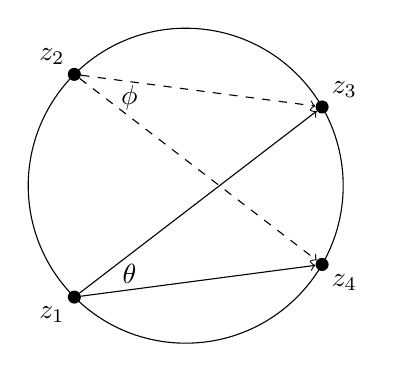
\begin{tikzpicture}
        \draw (0,0) circle [radius=2];
        \node [circle,fill,scale=0.5] (1) at ({-sqrt(2)},{-sqrt(2)}) {};
        \node [circle,fill,scale=0.5] (2) at ({-sqrt(2)},{sqrt(2)}) {};
        \node [circle,fill,scale=0.5] (3) at ({sqrt(3)},1) {};
        \node [circle,fill,scale=0.5] (4) at ({sqrt(3)},-1) {};
        \draw [->] (1) node [below left] {$z_1$} --
        (3) node [above right] {$z_3$};
        \draw [->] (1) -- (4) node [below right] {$z_4$};
        \draw [->,dashed] (2) node [above left] {$z_2$} -- (3);
        \draw [->,dashed] (2) -- (4);
        \node at ({-sqrt(2)+0.7},{-sqrt(2)+0.3}) {$\o$};
        \node at ({-sqrt(2)+0.7},{sqrt(2)-0.3}) {$\p$};
      \end{tikzpicture}

      But $\o=\p$

      $\therefore z_1,z_2,z_2,z_4$ lie on a circle.
      
    \item Case 3: $s<0$
      \begin{eqnarray*}
        \arg{s} &=& \arg(z_1,z_2,z_3,z_4) \\
        &=& \arg\left[\frac{(z_1-z_3)(z_2-z_4)}{(z_1-z_4)(z_2-z_3)}\right] \\
        &=& \arg\left[\frac{z_1-z_3}{z_1-z_4}\right]+
        \arg\left[\frac{z_2-z_4}{z_2-z_3}\right] \\
        &=& \arg\left[\frac{z_3-z_1}{z_4-z_1}\right]+
        \arg\left[\frac{z_4-z_2}{z_3-z_2}\right] \\
      \end{eqnarray*}
      But $\arg{s}=\pi$, so
      \[\arg\left[\frac{z_3-z_1}{z_4-z_1}\right]+
      \arg\left[\frac{z_4-z_2}{z_3-z_2}\right] = \pi\]

      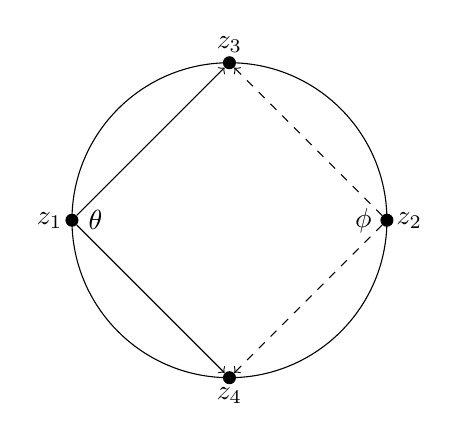
\begin{tikzpicture}
        \draw (0,0) circle [radius=2];
        \node [circle,fill,scale=0.5] (1) at (-2,0) {};
        \node [circle,fill,scale=0.5] (2) at (2,0) {};
        \node [circle,fill,scale=0.5] (3) at (0,2) {};
        \node [circle,fill,scale=0.5] (4) at (0,-2) {};
        \draw [->] (1) node [left] {$z_1$} -- (3) node [above] {$z_3$};
        \draw [->] (1) -- (4) node [below] {$z_4$};
        \draw [->,dashed] (2) node [right] {$z_2$} -- (3);
        \draw [->,dashed] (2) -- (4);
        \node at (-1.7,0) {$\o$};
        \node at (1.7,0) {$\p$};
      \end{tikzpicture}

      But $\o+\p=\pi$

      $\therefore z_1,z_2,z_2,z_4$ lie on a circle.
    \end{description}
    
  \item $\impliedby$ Assume $z_1,z_2,z_2,z_4$ lie on a circle
  \end{description}
\end{theproof}

\begin{corollary}
  A LFT maps a circle (or line) onto a circle (or line).
\end{corollary}

\begin{theproof}
  Let $w=s(z)$ be a LFT \\
  Assume $z_1,z_2,z_3,z_4$ lie on a circle \\
  $(z_1,z_2,z_3,z_4)\in\R$ \\
  But $(z_1,z_2,z_3,z_4)=(w_1,w_2,w_3,w_4)$ \\
  So $(w_1,w_2,w_3,w_4)\in\R$ \\
  $\therefore w_1,w_2,w_3,w_4$ lie on a circle.
\end{theproof}

\end{document}
